\chapter{考察}\label{cha:Discussion}

本章では、第5章で得られた評価結果に基づき、提案プロンプトの有用性と特性について考察する。
具体的には、手法A(手動作成)および手法B(自由プロンプト)との比較を通じて、手法C(提案プロンプト)が章立ての品質に与える影響を分析する。
また、プロンプトの構成要素が果たした役割や、対象システムの複雑さが生成結果に与える影響についても議論する。
さらに、関連研究についても述べる。

\section{関連研究}

本節では、本研究と関連する研究について述べる。

Zhu氏らは、LLMを活用して、要求定義書や要件定義書、会議の議事録といった自然言語で書かれたドキュメントから、ソフトウェア要求仕様書(本研究でのシステム仕様書に相当)を自動生成するエージェントであるREQINONEを開発した\cite{reference}。
REQINONEは、入力となるドキュメントから情報を要約、抽出、整形して、あらかじめ用意された章立てテンプレートの、どの章、節に整形した情報を配置するかを決めることで、ソフトウェア要求仕様書の自動生成を実現している。
したがって、このエージェント内では、章立ての自動生成は行われていない。
つまり、テンプレートとなる章立てを人間が事前に用意する必要がある。

一方、本研究で提案するプロンプトは、章立てそのものを自動生成することを目的としている。
% REQINONEが用意された章立てテンプレートに詳細な文書から情報を要約、抽出し、適切な章、節に配置するのに対し、
% 本研究では、システム名と短文のシステム概要のみを入力として、
% 対象システムに適した章立てを生成する。
% これにより、開発の初期段階において、詳細な要求定義書や要件定義書、会議の議事録が存在しない状況でも、
% システム仕様書の骨格となる章立てを作成できる点が本研究の特長である。

% また、REQINONEは膨大な入力文書を必要とするため、情報が十分に揃った状況での利用を想定している。
% 一方、本研究のプロンプトは最小限の情報で章立てを生成できるため、
% プロジェクトの初期段階から活用でき、REQINONEとは補完的な関係にあると言える。
したがって、REQINONEと本研究で提案するプロンプトは、補完的な関係にあると言える。

% 上前氏らは、LLMを用いてマニュアルの目次(章立て)を自動生成のための情報分類と順序付けの手法を提案している。
% 上前氏らの手法では、目次作成のプロセスをページ分類選択と順序付けの2段階に分け、目次の生成を行っている。
% 入力には、ページと呼ばれるマニュアルの目次に掲載されるページ集合を入力としている。
% 上前氏らの研究におけるページとは、タイトルと本文の組み合わせである。

\section{章立ての評価者による評価結果に対する分析}

% \addtocontents{toc}{\protect\setcounter{tocdepth}{1}}
\subsection{手法A(手動作成)と手法C(提案プロンプト)で作成した章立ての評価結果の分析}
% \addtocontents{toc}{\protect\setcounter{tocdepth}{2}}

実験結果より、手法C(提案プロンプト)は、手法A(手動作成)と比較して、多くの評価項目で高い点数を獲得した(表\ref{tb:bmp}、表\ref{tb:cloud}参照)。
特に「網羅性」「可読性」「独自性」の項目において、優位性がある。

BMP画像分割アプリの結果(表\ref{tb:bmp})において、手法C(提案プロンプト)は評価項目のすべてにおいて、手法A(手動作成)を上回った。特に、手法A(手動作成)の網羅性が3.6点であったのに対し、手法C(提案プロンプト)は4.3点と高い評価を得た。
これは、システム開発の経験が浅い作成者は、「用語定義」や「テスト観点」といった項目を漏らしてしまう傾向があり、被験者Aの結果もこれを裏付けている。
実際に、評価者からは手法A(手動作成)に対し「書くべきことが書けていない」や「シンプル」といった、内容の不足や具体性の欠如を指摘するコメントがあった。
一方、提案プロンプトを用いることで、ベース章立てテンプレートと役割付与により、抜け漏れが少ない章立てを生成したと考える。
実際に手法C(提案プロンプト)に対しては、「一番整理されている」「構成が分かりやすくていい」といった、論理的で整理された構造を高く評価するコメントがあった。

クラウド型電子契約サービスの結果(表\ref{tb:cloud})においては、論理性以外のすべての評価項目で手法A(手動作成)を上回った。特に「独自性」において手法C(提案プロンプト)(3.7点)は手法A(手動作成)(2.8点)を大きく上回った。
手動作成では、対象とするシステムに対する知識が不足している場合(例えばクラウドサービスのセキュリティ要件や電子署名の法的要件など)、システム固有の詳細な項目を書き出すことが困難である。
一方、提案プロンプトを用いることで、LLMが持つ広範な知識を活用し、作成者の知識の不足を補完することで、独自性の高い章立てが可能となったと考察する。

クラウド型電子契約サービスにおいても、手法A(手動作成)に対し評価者から「粒度が荒すぎる上に項目として不足箇所が多い」「章立てが荒く、記載が不足している」というコメントがあったのに対し、手法C(提案プロンプト)は「必要なことが書かれている」「拡張しやすそう」という評価を得ており、提案プロンプトが網羅性と将来の拡張性の両立に寄与していることを示した。
これは、提案プロンプトのベース章立てテンプレートと出力指示により、章、節、項の階層構造が明確になり、読みやすく整理された構成を出力した結果であると考察する。
実際に「可読性」に関しても、手法C(提案プロンプト)はBMP画像分割アプリの章立てで4.2点、クラウド型電子契約サービスの章立てで3.8点と、手法A(手動作成)(BMP: 3.4点、クラウド: 3.6点)を上回っている。

% 以上のことから、提案プロンプトは、特に仕様書作成の経験が浅い作成者にとって、手動作成よりも高品質でバランスの取れた章立てを作成するための強力な支援ツールとなると言える。

\subsection{手法B(自由プロンプト)と手法C(提案プロンプト)で作成した章立ての評価結果の分析}
手法B(自由プロンプト)と、手法C(提案プロンプト)の比較からは、提案プロンプトの「安定性」と「品質の均一化」の効果が確認できた。

BMP画像分割アプリにおいて、手法B(自由プロンプト)(被験者C)は網羅性で4.8点という非常に高い点数を記録したが、拡張性は2.8点であった。
また、手法B(自由プロンプト)には複数の評価者から「冗長」というコメントがあった。
これは、「網羅性」や「独自性」が高い一方で、実務上の使い勝手や情報の整理状況において課題があることを示している。
一方で、手法C(提案プロンプト)は網羅性4.3点、拡張性3.8点と、両項目で高い評価を得ており、評価者からは、「一番バランスが良い」「一番拡張性は高く使い勝手は一番よさそう」という評価を得ている。
これは、自由プロンプト特有の「過剰な生成」による拡張性の低下を、提案プロンプトの制約(テンプレートやシステム仕様書の定義)が適切に抑制し、品質の安定化に寄与した結果であると言える。

クラウド型電子契約サービスにおいて、手法B(自由プロンプト)(被験者D)は粒度の適切さで4.8点、独自性で4.6点と極めて高い評価を得た。
これは、被験者Dが少ない制約で自由度を与えたことで、LLMがその能力を最大限に発揮し、クラウドサービス特有の要件を網羅した詳細な仕様書を作成できた例である。
% これに対し、手法C(提案プロンプト)は粒度の適切さ3.4点、独自性3.7点と、手法B(自由プロンプト)には及ばない項目もあった。
% しかし、手法B(自由プロンプト)の論理性や構造的整合性が3点台後半から4.0点と評価者によってばらつきが見られたのに対し、手法C(提案プロンプト)は概ね安定した評価を得ている。

また、手法B(自由プロンプト)において、BMP画像分割アプリの合計点数は34.2点、クラウド型電子契約サービスの合計点数は38.0点であり、その差は3.8点であった。
一方で、手法C(提案プロンプト)の合計点数はそれぞれ36.2点、33.9点であり、その差は2.3点であった。
これは、手法B(自由プロンプト)は対象とするシステムに応じて、品質のばらつきが大きく、手法C(提案プロンプト)は品質のばらつきが少ないことを示している。


\section{IEEE830に基づく章立ての評価とその分析}

表\ref{tb:ieeee}は、IEEE830がシステム仕様書の章立てに含むことを推奨する項目(図\ref{fig:ieee830}参照)と評価実験で作成した章立て(\ref{sec:evaluation_results}節を参照)を比較し、各章立てがIEEE830がシステム仕様書の章立てに含むことを推奨する項目をどれだけ満たしているかを示した表である。
この表から、BMP画像分割アプリを対象として手法Aで作成した章立て(図\ref{fig:A_chapter_structure_of_bmp_app}参照)は、IEEE830がシステム仕様書の章立てに含むことを推奨する項目を36項目中11項目(30.6\%)満たしていることが分かる。
また、BMP画像分割アプリを対象として手法Bで作成した章立て(図\ref{fig:B_chapter_structure_of_bmp_app}参照)は、36項目中13項目(36.1\%)満たしていることが分かる。
また、BMP画像分割アプリを対象として被験者Bが手法Cで作成した章立て(図\ref{fig:C_chapter_structure_of_bmp_app_1})は、36項目中16項目(44.4\%)満たしていることが分かる。
また、BMP画像分割アプリを対象として被験者Dが手法Cで作成した章立て(図\ref{fig:C_chapter_structure_of_bmp_app_2})は、36項目中16項目(44.4\%)満たしていることが分かる。
また、クラウド型電子契約サービスを対象として手法Aで作成した章立て(図\ref{fig:A_chapter_structure_of_cloud_contract_system}参照)は、IEEE830がシステム仕様書の章立てに含むことを推奨する項目を36項目中14項目(38.9\%)満たしていることが分かる。
また、クラウド型電子契約サービスを対象として手法Bで作成した章立て(図\ref{fig:B_chapter_structure_of_cloud_contract_system}参照)は、36項目中26項目(72.2\%)満たしていることが分かる。
また、クラウド型電子契約サービスを対象として被験者Aが手法Cで作成した章立て(図\ref{fig:C_chapter_structure_of_cloud_contract_system_1})は、36項目中24項目(66.7\%)満たしていることが分かる。
また、クラウド型電子契約サービスを対象として被験者Cが手法Cで作成した章立て(図\ref{fig:C_chapter_structure_of_cloud_contract_system_2})は、36項目中22項目(61.1\%)満たしていることが分かる。

この結果から、手法C(提案プロンプト)は、手法A(手動作成)と比較して、IEEE830がシステム仕様書の章立てに含むことを推奨する項目を多く満たしていることが分かる。
また、手法C(提案プロンプト)のBMP画像分割アプリとクラウド型電子契約サービスの差は、8項目であるのに対し、手法B(自由プロンプト)の差は13項目である。
したがって、手法C(提案プロンプト)は、手法B(自由プロンプト)と比較して、対象システムの違いによる章立ての品質のばらつきが少ないことが分かる。

また、手法C(提案プロンプト)は、BMP画像分割アプリにおいて、平均の網羅率が44.4\%であり、クラウド型電子契約サービスにおいては、平均の網羅率が63.9\%である。
今回の提案プロンプトの「システム仕様書の定義」の中に目的として、「システムテスト担当者がテスト項目を作るために参照する文書」という項目を入れたが、これらの網羅率の数値は、テスト設計の網羅性という観点において、不十分な数値だと考える。
したがって、テスト設計の網羅性を向上させるために、「システム仕様書の定義」の記述を改善する必要があると考察する。

\begin{table}[tp]
  \centering
  \caption{IEEE830の章立てに含むことが推奨される項目と評価実験で作成した章立ての比較}
  \label{tb:ieeee}
%   \footnotesize
%   \renewcommand{\arraystretch}{1.2}
  \scriptsize
  \renewcommand{\arraystretch}{0.7}
  \setlength{\tabcolsep}{2pt}
  \begin{tabular}{|l|c|c|c|c|c|c|c|c|c|}
    \hline
    \textbf{仕様書の章立て項目} &\begin{tabular}{c} \textbf{手法A}\\\textbf{(BMP)} \\ \end{tabular}& \begin{tabular}{c} \textbf{手法B}\\\textbf{(BMP)} \\ \end{tabular}& \begin{tabular}{c} \textbf{手法C}\\\textbf{(BMP,}\\\textbf{被験者B)} \\ \end{tabular}& \begin{tabular}{c} \textbf{手法C}\\\textbf{(BMP,}\\\textbf{被験者D)} \\ \end{tabular}& \begin{tabular}{c} \textbf{手法A}\\\textbf{(電子契約)} \\ \end{tabular}& \begin{tabular}{c} \textbf{手法B}\\\textbf{(電子契約)} \\ \end{tabular}& \begin{tabular}{c} \textbf{手法C}\\\textbf{(電子契約,}\\\textbf{被験者A)} \\ \end{tabular}& \begin{tabular}{c} \textbf{手法C}\\\textbf{(電子契約,}\\\textbf{被験者C)} \\ \end{tabular}\\ \hline
    1. はじめに & 〇& 〇& 〇& 〇& 〇& 〇& 〇& 〇 \\ \hline
    \forceindent1.1 本書の目的 & 〇& 〇& 〇& 〇& 〇& 〇& 〇& 〇 \\ \hline
    \forceindent1.2 対象範囲 & & & 〇& 〇& 〇& 〇& 〇& 〇 \\ \hline
    \forceindent1.3 用語定義・略語 &〇 & 〇& 〇& 〇&〇 & & & \\ \hline
    \forceindent1.4 本書の構成 & &〇 &〇 &〇 & &〇 & 〇&〇 \\ \hline
    2. システム概要 &〇 & 〇& 〇& 〇&〇 & 〇& 〇& 〇\\ \hline
    \forceindent2.1 システムの全体像 & & 〇& 〇& 〇& &〇 &〇 & 〇\\ \hline
    \forceindent\forceindent2.1.1 システム間インターフェース & & & & & & & & \\ \hline
    \forceindent\forceindent2.1.2 画面インターフェース & & & & & & & & \\ \hline
    \forceindent\forceindent2.1.3 ハードウェア構成 & & & & & 〇& &〇 & \\ \hline
    \forceindent\forceindent2.1.4 ソフトウェア構成 &〇 & & & & 〇& 〇& 〇&〇 \\ \hline
    \forceindent\forceindent2.1.5 ネットワーク構成 &〇 & & & & 〇& 〇& 〇&〇 \\ \hline
    \forceindent\forceindent2.1.6 リソース制約 & & & & & & & & \\ \hline
    \forceindent\forceindent2.1.7 運用環境 &〇 & 〇&〇 &〇 & & 〇& 〇&〇 \\ \hline
    \forceindent\forceindent2.1.8 設置条件 & & & & & & & & \\ \hline
    \forceindent2.2 システムの主な機能 &〇 &〇 &〇 &〇 &〇 & 〇& 〇& 〇\\ \hline
    \forceindent2.3 想定利用者 & & & 〇& 〇& & 〇& 〇&〇 \\ \hline
    \forceindent2.4 制約事項 & &〇 &〇 &〇 & &〇 & 〇& 〇\\ \hline
    \forceindent2.5 前提条件および依存関係 & & &〇 & 〇& & 〇& 〇& 〇\\ \hline
    \forceindent2.6 将来対応事項 & & 〇& & & & & 〇& \\ \hline
    3. 詳細要件 & & &〇 & 〇&〇 & & 〇& 〇\\ \hline
    \forceindent3.1 外部インターフェース仕様 & & & & & &〇 &〇 & \\ \hline
    \forceindent3.2 機能要件 &〇 &〇 &〇 &〇 &〇 &〇 &〇 &〇 \\ \hline
    \forceindent3.3 性能要件 & &〇 &〇 &〇 & &〇 &〇 &〇 \\ \hline
    \forceindent3.4 データベース要件 &〇 & & & & &〇 &〇 & 〇\\ \hline
    \forceindent3.5 設計上の制約事項 & & & & &〇 & & & \\ \hline
    \forceindent3.6 システム品質特性 & & & & & &〇 & & \\ \hline
    \forceindent\forceindent3.6.1 信頼性 & & & & & & 〇& & \\ \hline
    \forceindent\forceindent3.6.2 可用性 & &  & & & & 〇& 〇&〇 \\ \hline
    \forceindent\forceindent3.6.3 セキュリティ &〇 &〇 &〇 &〇 &〇 &〇 & 〇& 〇\\ \hline
    \forceindent\forceindent3.6.4 保守性 & & & & & & 〇&〇 & \\ \hline
    \forceindent\forceindent3.6.5 移植性 & & & & &〇 &〇 & & \\ \hline
    \forceindent3.7 その他の要件 & & &〇 & 〇&〇 &〇 & 〇& 〇\\ \hline
    4. 参考資料 & & & & & &〇 & &〇 \\ \hline
    \forceindent4.1 索引 & & & & & & & & \\ \hline
    \forceindent4.2 付録 &〇 &〇 & & &〇 & &〇 & 〇\\ \hline
    \textbf{合計} & \textbf{11}& \textbf{13}& \textbf{16}& \textbf{16}& \textbf{14}& \textbf{26}& \textbf{24}& \textbf{22}\\ \hline
  \end{tabular}
\end{table}

\section{プロンプトに対する分析}
\subsection{提案プロンプトの構成要素の寄与}

% 提案するプロンプトの構成要素が生成結果に与える影響を確認するため、図\ref{fig:base_prompt}をベースプロンプトとして、図\ref{fig:prompt_structure}に示した各構成要素のみを追加したプロンプト5つを作成し、それぞれを用いて章立てを生成した。
提案プロンプトの構成要素が生成結果に与える影響を確認するため、「開発するシステム情報」と「出力指示」からなるプロンプトをベースプロンプトとして作成する。
そして、ベースプロンプトに図\ref{fig:prompt_structure}に示したそれぞれの構成要素のみを追加したプロンプトを5つ作成し、それぞれを用いて章立てを生成する。

図\ref{fig:base_prompt}に、クラウド型電子契約サービスを対象としたベースプロンプトを示す。
なお、ベースプロンプトに「開発するシステム情報」を含む理由は、章立ての生成に最低限必要な情報であるためであり、出力指示を含む理由は、章立ての生成に最低限必要な指示と生成結果に章立て以外のものを含まないようにするためである。

\begin{figure}[tp]
\begin{tcolorbox}[
  colback=white,
  colframe=blue,
  fonttitle=\bfseries
]
\footnotesize
\ttfamily
\fontsize{8}{9}\selectfont
\begin{verbatim}
【開発するシステム情報】
- システム名：クラウド型電子契約サービス
- 概要：PDF技術を活かした電子契約／ワークフロー、それらに付随する文書管理、及びユーザー管理機能を持つクラウドサービス

【出力指示】
・上記情報に基づき、開発するシステムのシステム仕様書に必要な章立てを出力してください。
・ここでいう章立ては、以下の内容を含みます。
　・章と節、章タイトル、節タイトル、項、項タイトル 
・出力形式は**マークダウンの番号付きリスト**としてください。 
・章名以外(目的・記述のポイントなど)は一切書かないでください。
\end{verbatim}
\end{tcolorbox}
\caption{ベースプロンプト}
\label{fig:base_prompt}
\end{figure}

図\ref{fig:base_prompt_outline}に、ベースプロンプトを用いて生成した章立てを示す。

\begin{figure}[tp]
\begin{tcolorbox}[
  colback=white,
  colframe=orange,
  fonttitle=\bfseries
]
\begin{multicols}{2}
\footnotesize
\ttfamily
\fontsize{7}{8}\selectfont
\begin{verbatim}
1. システム概要
   1.1 システム目的
   1.2 システム範囲
   1.3 用語定義
   1.4 前提条件・制約事項

2. 全体構成
   2.1 システムアーキテクチャ
   2.2 構成要素一覧
   2.3 外部システム連携概要
   2.4 ネットワーク構成

3. 機能要件
   3.1 電子契約機能
   3.2 ワークフロー機能
   3.3 文書管理機能
   3.4 ユーザー管理機能
   3.5 管理者機能

4. 画面仕様
   4.1 画面一覧
   4.2 画面遷移図
   4.3 各画面仕様

5. データ仕様
   5.1 データモデル
   5.2 エンティティ定義
   5.3 データ項目定義
   5.4 データ保持方針

6. インターフェース仕様
   6.1 外部連携インターフェース
   6.2 API仕様
   6.3 ファイル入出力仕様

7. セキュリティ仕様
   7.1 認証・認可
   7.2 アクセス制御
   7.3 ログ管理
   7.4 データ暗号化

8. 非機能要件
   8.1 性能要件
   8.2 可用性要件
   8.3 拡張性要件
   8.4 運用性要件

9. 運用・保守仕様
   9.1 運用フロー
   9.2 バックアップ・リストア
   9.3 障害対応
   9.4 監視仕様

10. テスト仕様
    10.1 テスト方針
    10.2 テスト項目一覧
    10.3 受入テスト基準

11. 付録
    11.1 用語集
    11.2 参考資料
    11.3 改訂履歴

\end{verbatim}
\end{multicols}
\end{tcolorbox}
\caption{ベースプロンプトによる章立て}
\label{fig:base_prompt_outline}
\end{figure}

図\ref{fig:only_role}に、ベースプロンプトに役割付与のみを加えたプロンプトを示す。
また、図\ref{fig:only_role_outline}に、図\ref{fig:only_role}に示したプロンプトを用いて生成した章立てを示す。

図\ref{fig:base_prompt_outline}と図\ref{fig:only_role_outline}を比較すると、役割付与の追加により、節の項目が増加し、より網羅的な章立てになっていることが分かる。
具体的には、ベースプロンプトでは節が41個であったのに対し、役割付与を追加すると節が50個になっている。
これは、役割付与が章立ての網羅性の向上に寄与していることを示している。

\begin{figure}[tp]
\begin{tcolorbox}[
  colback=white,
  colframe=blue,
  fonttitle=\bfseries
]
\footnotesize
\ttfamily
\fontsize{8}{9}\selectfont
\begin{verbatim}
あなたはシステム仕様書作成の専門アシスタントです。


【開発するシステム情報】
- システム名：クラウド型電子契約サービス
- 概要：PDF技術を活かした電子契約／ワークフロー、それらに付随する文書管理、及びユーザー管理機能を持つクラウドサービス

【出力指示】
・上記情報に基づき、開発するシステムのシステム仕様書に必要な章立てを出力してください。
・ここでいう章立ては、以下の内容を含みます。
　・章と節、章タイトル、節タイトル、項、項タイトル 
・出力形式は**マークダウンの番号付きリスト**としてください。 
・章名以外(目的・記述のポイントなど)は一切書かないでください。
\end{verbatim}
\end{tcolorbox}
\caption{ベースプロンプトに役割付与のみを加えたプロンプト}
\label{fig:only_role}
\end{figure}



\begin{figure}[tp]
\begin{tcolorbox}[
  colback=white,
  colframe=orange,
  fonttitle=\bfseries
]
\begin{multicols}{2}
\footnotesize
\ttfamily
\fontsize{7}{8}\selectfont
\begin{verbatim}
1. システム概要
   1.1 目的
   1.2 適用範囲
   1.3 用語定義
   1.4 参照資料
   1.5 前提条件
   1.6 制約事項

2. 全体構成
   2.1 システム全体像
   2.2 システム構成図
   2.3 ネットワーク構成
   2.4 ソフトウェア構成
   2.5 ハードウェア構成

3. 機能仕様
   3.1 ユーザー管理機能
   3.2 文書管理機能
   3.3 電子契約機能
   3.4 ワークフロー機能
   3.5 通知機能
   3.6 検索・参照機能
   3.7 ログ管理機能
   3.8 権限管理機能

4. 画面仕様
   4.1 画面一覧
   4.2 画面遷移図
   4.3 画面レイアウト

5. データ仕様
   5.1 データモデル
   5.2 ER図
   5.3 テーブル定義
   5.4 インデックス定義
   5.5 データ保持ポリシー

6. 外部インターフェース仕様
   6.1 外部システム連携
   6.2 API仕様
   6.3 ファイル連携仕様

7. 非機能要件
   7.1 性能要件
   7.2 可用性要件
   7.3 拡張性要件
   7.4 セキュリティ要件
   7.5 バックアップ・リカバリ要件

8. 運用・保守仕様
   8.1 運用体制
   8.2 監視仕様
   8.3 障害対応
   8.4 バージョン管理
   8.5 保守対応

9. テスト仕様
   9.1 テスト方針
   9.2 テスト項目
   9.3 テスト環境
   9.4 受入テスト基準

10. セキュリティ仕様
    10.1 認証方式
    10.2 認可方式
    10.3 通信暗号化
    10.4 ログ監査

11. 制限事項
    11.1 システム制限
    11.2 運用上の制限

\end{verbatim}
\end{multicols}
\end{tcolorbox}
\caption{役割付与のみを加えたプロンプトによる章立て}
\label{fig:only_role_outline}
\end{figure}

図\ref{fig:only_outline}に、図\ref{fig:base_prompt}のベースプロンプトにベースの章立てのみを加えたプロンプトを示す。
また、図\ref{fig:only_outline_outline}に、図\ref{fig:only_outline}に示したプロンプトを用いて生成した章立てを示す。

図\ref{fig:base_prompt_outline}と図\ref{fig:only_outline_outline}を比較すると、ベースの章立てを追加したことにより、「1.概要」、「4.システム基本条件」のように、章タイトルがテンプレートに沿った命名になっていることが分かる。
これは、評価項目の命名の適切さにおいて、BMP画像分割アプリで4.1点(表\ref{tb:bmp})、電子契約サービスで3.9点(表\ref{tb:cloud})という高い評価を得た要因になっていると考える。
一方で、図\ref{fig:only_role_outline}に示した役割付与のみを行った場合と図\ref{fig:only_outline_outline}を比較すると、役割付与のみを追加した場合の章立てには、9章に「テスト仕様」があるが、ベースの章立てを追加した場合の章立てには、「テスト仕様」は存在しない。
これは、ベースの章立てを与えることにより、テンプレートに含まれていない項目がLLMによって生成されにくくなる可能性があることを示唆している。

\begin{figure}[tp]
\begin{tcolorbox}[
  colback=white,
  colframe=blue,
  fonttitle=\bfseries
]
\footnotesize
\ttfamily
\fontsize{8}{9}\selectfont
\begin{verbatim}
【ベース章立てテンプレート(参考)】
1. 概要
 1.1.目的
 1.2.システム概要
 1.3.適用範囲
2. システム基本条件
 2.1.稼働条件
 2.2.他システムインターフェース
 2.3.性能条件
 2.4.拡張条件
 2.5.継承条件
 2.6.以降環境
3. システム構成
 3.1.ハードウェア構成及びネットワーク構成
 3.2.ソフトウェア構成
4. システムの機能
 4.1.機能構成
 4.2.個別機能概要
5. システムの運用
 5.1.運用方法
 5.2.各業務(機能)の運用
 5.3.障害時の運用
6.セキュリティ
7.安全設計
8.データ仕様
 8.1.コード体系
 8.2.データベース
 8.3.ファイル
 8.4.入出力データ
 8.5.メッセージ
9.付帯事項

※ベース章立てはあくまで参考です。必要に応じて章の追加・削除・順序変更を行って、漏れなく体系的な章立てを作成してください。

【開発するシステム情報】
- システム名：クラウド型電子契約サービス
- 概要：PDF技術を活かした電子契約／ワークフロー、それらに付随する文書管理、及びユーザー管理機能を持つクラウドサービス

【出力指示】
・上記情報に基づき、開発するシステムのシステム仕様書に必要な章立てを出力してください。
・ここでいう章立ては、以下の内容を含みます。
　・章と節、章タイトル、節タイトル、項、項タイトル 
・出力形式は**マークダウンの番号付きリスト**としてください。 
・章名以外(目的・記述のポイントなど)は一切書かないでください。

\end{verbatim}
\end{tcolorbox}
\caption{ベースプロンプトにベースの章立てのみを加えたプロンプト}
\label{fig:only_outline}
\end{figure}

\begin{figure}[tp]
\begin{tcolorbox}[
  colback=white,
  colframe=orange,
  fonttitle=\bfseries
]
\begin{multicols}{2}
\footnotesize
\ttfamily
\fontsize{7}{8}\selectfont
\begin{verbatim}
1. 概要
   1.1. 目的
   1.2. システム概要
   1.3. 用語定義
   1.4. 適用範囲

2. 関連資料・前提条件
   2.1. 関連法規・ガイドライン
   2.2. 前提条件
   2.3. 制約条件

3. システム全体構成
   3.1. サービス全体構成
   3.2. ハードウェア構成及びネットワーク構成
   3.3. ソフトウェア構成
   3.4. 外部サービス構成

4. システム基本条件
   4.1. 稼働条件
   4.2. 性能条件
   4.3. 可用性条件
   4.4. 拡張条件
   4.5. 移行条件

5. システム機能要件
   5.1. 機能構成
   5.2. ユーザー管理機能
     5.2.1. ユーザー登録・変更・削除
     5.2.2. ロール・権限管理
     5.2.3. 認証・認可
   5.3. 電子契約機能
     5.3.1. 契約書作成・アップロード
     5.3.2. 署名依頼ワークフロー
     5.3.3. 電子署名・タイムスタンプ付与
     5.3.4. 署名進捗管理
   5.4. ワークフロー機能
     5.4.1. 承認経路設定
     5.4.2. 承認・差戻し・却下
   5.5. 文書管理機能
     5.5.1. 文書保管
     5.5.2. 検索・閲覧
     5.5.3. バージョン管理
   5.6. 通知機能
     5.6.1. メール通知
     5.6.2. 画面通知
   5.7. ログ管理機能
     5.7.1. 操作ログ
     5.7.2. 監査ログ

6. 外部システムインターフェース
   6.1. 外部認証基盤連携
   6.2. 外部署名サービス連携
   6.3. 外部ストレージ連携
   6.4. API連携

7. 非機能要件
   7.1. 性能要件
   7.2. 可用性要件
   7.3. 信頼性要件
   7.4. 拡張性要件
   7.5. 運用保守性要件

8. セキュリティ要件
   8.1. 認証方式
   8.2. アクセス制御
   8.3. データ暗号化
   8.4. 通信暗号化
   8.5. 監査証跡
   8.6. 脆弱性対策

9. データ仕様
   9.1. コード体系
   9.2. データベース設計
     9.2.1. エンティティ一覧
     9.2.2. ER図
   9.3. ファイル仕様
   9.4. 入出力データ仕様
   9.5. メッセージ仕様

10. 運用設計
    10.1. 運用方法
    10.2. 業務運用
    10.3. 障害時運用
    10.4. バックアップ・リストア
    10.5. 監視

11. 移行設計
    11.1. データ移行
    11.2. 移行手順
    11.3. 移行後確認

12. 安全設計

13. 付帯事項

\end{verbatim}
\end{multicols}
\end{tcolorbox}
\caption{ベースの章立てのみを加えたプロンプトによる章立て}
\label{fig:only_outline_outline}
\end{figure}

図\ref{fig:only_definition}に、図\ref{fig:base_prompt}のベースプロンプトにシステム仕様書の定義のみを加えたプロンプトを示す。
また、図\ref{fig:only_definition_outline}に、図\ref{fig:only_definition}に示したプロンプトによる章立てを示す。

図\ref{fig:base_prompt_outline}と図\ref{fig:only_definition_outline}を比較すると、システム仕様書の定義のみを加えたプロンプトにより、システム仕様書の定義内に記載されている外部仕様のみ記載、画面仕様と操作フローのみ含めるといった制約により、網羅性や独自性が損なわれていることが分かる。
具体的には、ベースプロンプトで作成した章立ては、章が11個、節が41個、項が0個であるのに対し、システム仕様書の定義のみを加えたプロンプトで作成した章立ては、章が6個、節が27個、項が31個である。すなわち、章、節の数が減少し、項の数が増加していることが分かる。
この結果から、提案プロンプトのシステム仕様書の定義が、評価実験において、網羅性と独自性において提案プロンプトが手法B(自由プロンプト)に劣った原因であると考察する。
また、図\ref{fig:only_definition_outline}の章立ては、エラーに関する章はあるものの、テスト観点での網羅性が低い章立てになっていると考える。
これは、システム仕様書の定義で、「テスト担当者：内部構造は知らず、仕様書に記載されたエラー条件に従ってテストを実施」という記述があることで、LLMがエラー条件を優先的に考慮したためであると考察できる。
しかし、評価実験の適合性に関する評価で、手法C(提案プロンプト)がBMP画像分割アプリで4.2点、クラウド型電子契約サービスにおいて3.9点という高い点数を獲得したのは、システム仕様書の定義が機能した結果であると言える。
このように、システム仕様書の定義は、網羅性や独自性を低下させる代わりに、適合性を高める効果があると言える。

\begin{figure}[tp]
\begin{tcolorbox}[
  colback=white,
  colframe=blue,
  fonttitle=\bfseries
]
\footnotesize
\ttfamily
\fontsize{8}{9}\selectfont
\begin{verbatim}
【システム仕様書の定義】
- 目的：
 ・プログラム作成者がシステムの仕様を理解し、設計・実装するための文書 
 ・システムテスト担当者がテスト項目を作るために参照する文書
- 対象読者:
 ・プログラム作成者：新人想定 
 ・テスト担当者：内部構造は知らず、仕様書に記載されたエラー条件に従ってテストを実施
- 記述スタイル：
 ・専門用語は必ず説明 
 ・初出の単語は必ず説明 
 ・システム概要は図を使って視覚的に理解できるようにする 
 ・図はユースケース図または独自の簡易図を使用し、必ずテキストで補足説明 
 ・用語や機能名は文書内で統一 
 ・データ型や制約が必要な場合は表形式で記載 
 ・外部仕様のみ記載(内部構造は書かない)
- システム要件：
 ・動作環境：OS、ハードウェア、ネットワーク 
 ・非機能要件：パフォーマンス、セキュリティ 
- 記述の粒度：
 ・画面レイアウトと操作フローのみ含める

【開発するシステム情報】
- システム名：クラウド型電子契約サービス
- 概要：PDF技術を活かした電子契約／ワークフロー、それらに付随する文書管理、及びユーザー管理機能を持つクラウドサービス

【出力指示】
・上記情報に基づき、開発するシステムのシステム仕様書に必要な章立てを出力してください。
・ここでいう章立ては、以下の内容を含みます。
　・章と節、章タイトル、節タイトル、項、項タイトル 
・出力形式は**マークダウンの番号付きリスト**としてください。 
・章名以外(目的・記述のポイントなど)は一切書かないでください。
\end{verbatim}
\end{tcolorbox}
\caption{ベースプロンプトにシステム仕様書の定義のみを加えたプロンプト}
\label{fig:only_definition}
\end{figure}


\begin{figure}[tp]
\begin{tcolorbox}[
  colback=white,
  colframe=orange,
  fonttitle=\bfseries
]
\begin{multicols}{2}
\footnotesize
\ttfamily
\fontsize{7}{8}\selectfont
\begin{verbatim}
1. システム概要
   1.1 システム全体像
   1.2 用語定義
   1.3 システム構成図
   1.4 ユースケース図

2. 動作環境および非機能要件
   2.1 動作環境
    2.1.1 対応OS
    2.1.2 ハードウェア要件
    2.1.3 ネットワーク要件
   2.2 非機能要件
    2.2.1 パフォーマンス要件
    2.2.2 セキュリティ要件

3. 画面仕様
   3.1 画面一覧
   3.2 ログイン画面
    3.2.1 画面レイアウト
    3.2.2 操作フロー
   3.3 ダッシュボード画面
    3.3.1 画面レイアウト
    3.3.2 操作フロー
   3.4 契約書作成画面
    3.4.1 画面レイアウト
    3.4.2 操作フロー
   3.5 ワークフロー設定画面
    3.5.1 画面レイアウト
    3.5.2 操作フロー
   3.6 文書管理画面
    3.6.1 画面レイアウト
    3.6.2 操作フロー
   3.7 ユーザー管理画面
    3.7.1 画面レイアウト
    3.7.2 操作フロー

4. 機能仕様
   4.1 電子契約機能
    4.1.1 契約書アップロード
    4.1.2 署名依頼送信
    4.1.3 署名実行
    4.1.4 契約完了処理
   4.2 ワークフロー機能
    4.2.1 承認ルート設定
    4.2.2 承認依頼送信
    4.2.3 承認／却下処理
   4.3 文書管理機能
    4.3.1 文書検索
    4.3.2 文書閲覧
    4.3.3 文書ダウンロード
   4.4 ユーザー管理機能
    4.4.1 ユーザー登録
    4.4.2 ユーザー編集
    4.4.3 ユーザー削除
    4.4.4 権限設定

5. 操作フロー
   5.1 契約書作成から署名完了までの操作フロー
   5.2 ワークフロー承認の操作フロー
   5.3 文書管理の操作フロー
   5.4 ユーザー管理の操作フロー

6. エラー条件およびエラーメッセージ
   6.1 共通エラー
   6.2 ログイン関連エラー
   6.3 契約書操作関連エラー
   6.4 ワークフロー関連エラー
   6.5 文書管理関連エラー
   6.6 ユーザー管理関連エラー
\end{verbatim}
\end{multicols}
\end{tcolorbox}
\caption{システム仕様書の定義のみを加えたプロンプトによる章立て}
\label{fig:only_definition_outline}
\end{figure}

図\ref{fig:only_output}に、図\ref{fig:base_prompt}のベースプロンプトに出力指示に、網羅性と自由度に関する指示を加えたプロンプトを示す。
また、図\ref{fig:only_output_outline}に、図\ref{fig:only_output}に示したプロンプトによる章立てを示す。

図\ref{fig:base_prompt_outline}と図\ref{fig:only_output_outline}を比較すると、図\ref{fig:only_output_outline}の章立ては、章、節、項の数が大幅に増加しており、網羅性、独自性の向上に寄与していると考える。
一方で、クラウド型電子契約サービスの章立ての手法C(提案プロンプト)における評価(表\ref{tb:cloud}参照)で粒度の適切さが3.4点と低い点数になった要因として、出力指示(網羅性と自由度に関する指示)によって、章立ての階層が深くなりすぎたことが考察できる。
これにより、評価者が粒度が細かすぎると判断し、粒度の適切さを低く評価した可能性がある。

\begin{figure}[tp]
\begin{tcolorbox}[
  colback=white,
  colframe=blue,
  fonttitle=\bfseries
]
\footnotesize
\ttfamily
\fontsize{8}{9}\selectfont
\begin{verbatim}
【開発するシステム情報】
- システム名：クラウド型電子契約サービス
- 概要：PDF技術を活かした電子契約／ワークフロー、それらに付随する文書管理、及びユーザー管理機能を持つクラウドサービス

【出力指示】
・上記情報に基づき、開発するシステムのシステム仕様書に必要な章立てを出力してください。
・ここでいう章立ては、以下の内容を含みます。
　・章と節、章タイトル、節タイトル、項、項タイトル 
・出力形式は**マークダウンの番号付きリスト**としてください。 
・章名以外(目的・記述のポイントなど)は一切書かないでください。
・章の追加や削除、順序の変更は自由に行って構いません。
・人間が考慮し忘れるような章立ても考えるのがあなたの役目です。考慮漏れが無いように、網羅性を高めてください。
\end{verbatim}
\end{tcolorbox}
\caption{ベースプロンプトに出力指示(網羅性と自由度の指示)を加えたプロンプト}
\label{fig:only_output}
\end{figure}

\begin{figure}[tp]
\begin{tcolorbox}[
  colback=white,
  colframe=orange,
  fonttitle=\bfseries
]
\begin{multicols}{2}
\footnotesize
\ttfamily
\fontsize{7}{8}\selectfont
\begin{verbatim}
1. はじめに
   1.1 目的
   1.2 適用範囲
   1.3 用語定義
   1.4 参照文書

2. システム概要
   2.1 システム全体像
   2.2 提供サービス概要
   2.3 想定利用シナリオ
   2.4 システム構成概要

3. システムアーキテクチャ
   3.1 全体アーキテクチャ構成
   3.2 論理構成図
   3.3 物理構成図
   3.4 採用技術スタック
   3.5 外部サービス構成

4. 機能要件
   4.1 電子契約機能
      4.1.1 契約書アップロード
      4.1.2 署名依頼フロー設定
      4.1.3 電子署名実行
      4.1.4 タイムスタンプ付与
      4.1.5 契約締結管理
      4.1.6 契約書ダウンロード／閲覧
   4.2 ワークフロー機能
      4.2.1 承認ルート設定
      4.2.2 承認依頼通知
      4.2.3 承認／却下処理
      4.2.4 進捗状況管理
   4.3 文書管理機能
      4.3.1 文書登録
      4.3.2 文書検索
      4.3.3 バージョン管理
      4.3.4 フォルダ管理
      4.3.5 アクセス権管理
   4.4 ユーザー管理機能
      4.4.1 ユーザー登録／編集／削除
      4.4.2 ロール管理
      4.4.3 組織管理
      4.4.4 認証／認可
   4.5 通知機能
      4.5.1 メール通知
      4.5.2 リマインド通知
   4.6 ログ管理機能
      4.6.1 操作ログ
      4.6.2 監査ログ
      4.6.3 ログ検索／出力

5. 画面仕様
   5.1 画面一覧
   5.2 画面遷移図
   5.3 各画面仕様

6. データ仕様
   6.1 データモデル
   6.2 ER図
   6.3 テーブル定義
   6.4 インデックス設計
   6.5 データ保持ポリシー

7. 外部連携仕様
   7.1 外部API連携
   7.2 Webhook仕様
   7.3 SSO連携
   7.4 タイムスタンプサービス連携

8. 非機能要件
   8.1 性能要件
   8.2 可用性要件
   8.3 拡張性要件
   8.4 セキュリティ要件
   8.5 運用性要件
   8.6 互換性要件

9. セキュリティ設計
   9.1 認証方式
   9.2 認可方式
   9.3 データ暗号化
   9.4 脆弱性対策
   9.5 監査対応

10. 運用設計
   10.1 運用体制
   10.2 バックアップ／リストア
   10.3 障害対応
   10.4 監視設計
   10.5 バージョン管理／リリース管理

11. テスト計画
   11.1 テスト方針
   11.2 テスト種別
   11.3 テスト環境
   11.4 テストデータ方針

12. 移行設計
   12.1 データ移行方針
   12.2 移行手順
   12.3 移行検証

13. 制約事項
   13.1 法令・規格準拠
   13.2 技術的制約
   13.3 運用上の制約

14. 将来拡張計画
   14.1 機能拡張想定
   14.2 外部連携拡張想定

\end{verbatim}
\end{multicols}
\end{tcolorbox}
\caption{ベースプロンプトに出力指示(網羅性と自由度の指示)を加えたプロンプトによる章立て}
\label{fig:only_output_outline}
\end{figure}

% 図\ref{fig:coverage}は、提案するプロンプトの各構成要素が、章、節、項の数にどのような影響を与えるかを示したグラフである。
% 図\ref{fig:coverage}から、役割付与、ベースの章立てテンプレートの追加、出力指示(網羅性と自由度の指示)の追加は、章立ての網羅性を高めることが分かる。
% 一方で、ベースプロンプトで作成された章立てと比較して、システム仕様書の定義を追加したプロンプトによって、章、節の数が減少し、項の数が増加することが分かる。
% これは、手法B(自由プロンプト)より手法C(提案プロンプト)の方が網羅性が低いという評価を受けた原因であることが分かる。

% \begin{figure}[tp]
%   \centering
%   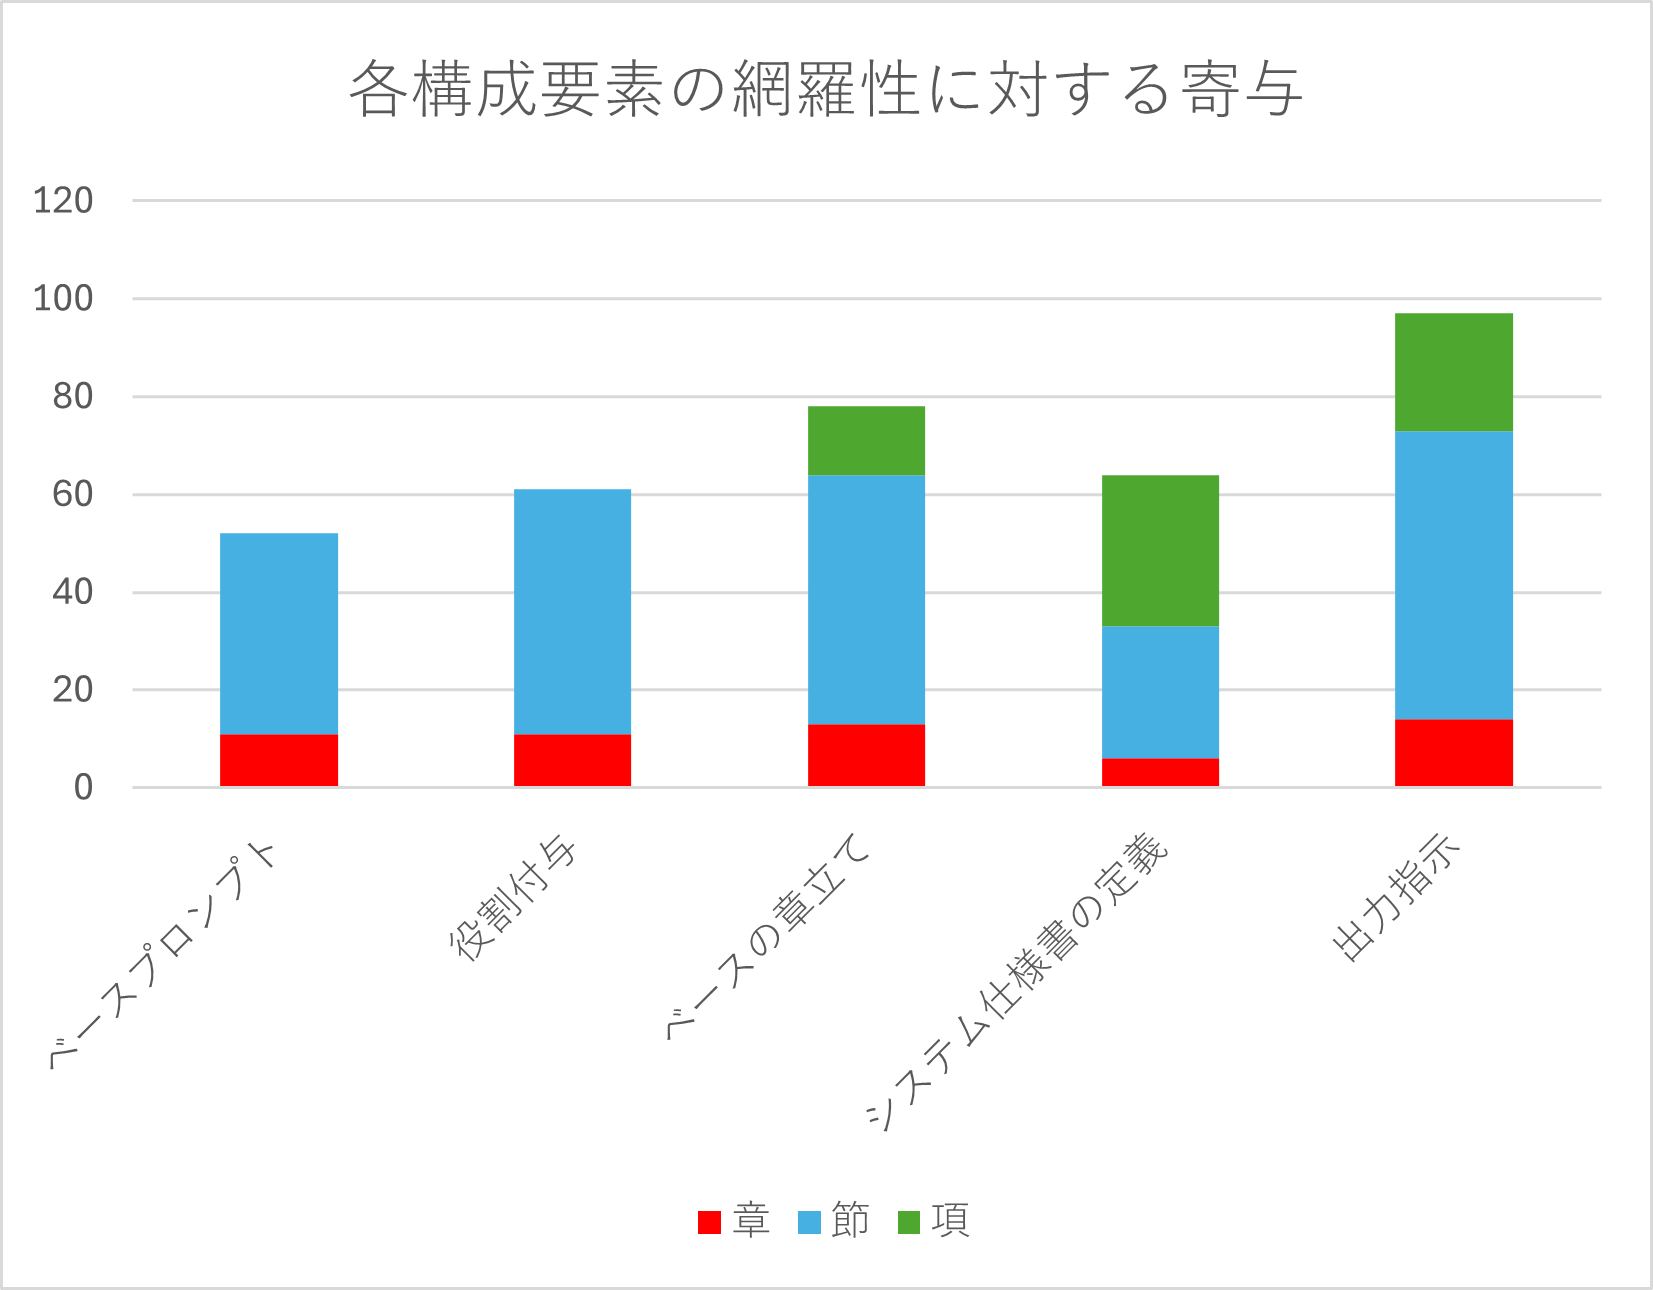
\includegraphics[width=0.8\textwidth]{images/網羅性.png}
%   \caption{各構成要素の網羅性に対する寄与}
%   \label{fig:coverage}
% \end{figure}

表\ref{tb:ieee}は、IEEE830がシステム仕様書の章立てに含むことを推奨する項目(図\ref{fig:ieee830}参照)と図\ref{fig:base_prompt_outline}、図\ref{fig:only_role_outline}、図\ref{fig:only_outline_outline}、図\ref{fig:only_definition_outline}、図\ref{fig:only_output_outline}に示した章立てを比較し、各プロンプトの構成要素がIEEE830がシステム仕様書の章立てに含むことを推奨する項目をどれだけ満たしているかを示した表である。
この表から、ベースプロンプト(図\ref{fig:base_prompt})による章立て(図\ref{fig:base_prompt_outline})は、IEEE830がシステム仕様書の章立てに含むことを推奨する項目を36項目中17項目満たしていることが分かる。
役割付与を追加したプロンプト(図\ref{fig:only_role})による章立て(図\ref{fig:only_role_outline})は、36項目中19項目満たしていることが分かる。
ベースの章立てテンプレートを追加したプロンプト(図\ref{fig:only_outline})による章立て(図\ref{fig:only_outline_outline})は、36項目中23項目満たしていることが分かる。
システム仕様書の定義を追加したプロンプト(図\ref{fig:only_definition})による章立て(図\ref{fig:only_definition_outline})は、36項目中11項目満たしていることが分かる。
出力指示(網羅性と自由度の指示)を追加したプロンプト(図\ref{fig:only_output})による章立て(図\ref{fig:only_output_outline})は、36項目中19項目満たしていることが分かる。

この結果からも、「システム仕様書の定義」は網羅性を低下させる要因であることが分かる。
一方で、「役割付与」、「ベースの章立て」、「出力指示」は網羅性の向上に寄与することが分かる。
特に、「ベースの章立て」は、網羅性に最も寄与することが分かる。

この結果から、網羅性の高い章立てを作成するためには、質の良い「ベースの章立て」を用意することが重要であると考察できる。
したがって、LLMとの対話を1回で終わらせるのではなく、1回目の生成結果の出力である章立てを、次回のプロンプトの「ベースの章立て」として再利用することで、章立てを段階的に洗練させる再帰的な手法が有効である可能性がある。


\begin{table}[tp]
  \centering
  \caption{IEEE830の章立てに含むことが推奨される項目と各プロンプト構成要素の対応}
  \label{tb:ieee}
%   \footnotesize
%   \renewcommand{\arraystretch}{1.2}
  \scriptsize
  \renewcommand{\arraystretch}{0.9}
  \setlength{\tabcolsep}{3pt}
  \begin{tabular}{|l|c|c|c|c|c|}
    \hline
    \textbf{仕様書の章立て項目} & \textbf{ベースプロンプトを追加} & \textbf{役割付与を追加} & \textbf{ベースの章立てを追加} & \textbf{仕様書の定義を追加} & \textbf{出力指示を追加} \\ \hline
    1. はじめに & & & & &〇 \\ \hline
    \forceindent1.1 本書の目的 & & &〇 & &〇 \\ \hline
    \forceindent1.2 対象範囲 &〇 & 〇& 〇& &〇 \\ \hline
    \forceindent1.3 用語定義・略語 &〇 & 〇& 〇& 〇&〇 \\ \hline
    \forceindent1.4 本書の構成 & & & & & \\ \hline
    2. システム概要 &〇 & 〇& 〇& 〇&〇 \\ \hline
    \forceindent2.1 システムの全体像 & 〇& 〇& 〇& 〇&〇 \\ \hline
    \forceindent\forceindent2.1.1 システム間インターフェース & & & & & \\ \hline
    \forceindent\forceindent2.1.2 画面インターフェース & & & & & \\ \hline
    \forceindent\forceindent2.1.3 ハードウェア構成 & & 〇& 〇& 〇& 〇\\ \hline
    \forceindent\forceindent2.1.4 ソフトウェア構成 & &〇 & 〇& & \\ \hline
    \forceindent\forceindent2.1.5 ネットワーク構成 &〇 &〇 &〇 &〇 & \\ \hline
    \forceindent\forceindent2.1.6 リソース制約 & & & & & \\ \hline
    \forceindent\forceindent2.1.7 運用環境 & & &〇 & & \\ \hline
    \forceindent\forceindent2.1.8 設置条件 & & & & & \\ \hline
    \forceindent2.2 システムの主な機能 &〇 &〇 &〇 &〇 &〇 \\ \hline
    \forceindent2.3 想定利用者 & & & & &〇 \\ \hline
    \forceindent2.4 制約事項 & 〇&〇 &〇 & & 〇\\ \hline
    \forceindent2.5 前提条件および依存関係 &〇 &〇 &〇 & & \\ \hline
    \forceindent2.6 将来対応事項 & & & & & 〇\\ \hline
    3. 詳細要件 & & &〇 & 〇&〇 \\ \hline
    \forceindent3.1 外部インターフェース仕様 &〇 &〇 &〇 & & \\ \hline
    \forceindent3.2 機能要件 &〇 &〇 &〇 &〇 &〇 \\ \hline
    \forceindent3.3 性能要件 &〇 &〇 &〇 &〇 &〇 \\ \hline
    \forceindent3.4 データベース要件 & & &〇 & & \\ \hline
    \forceindent3.5 設計上の制約事項 & & & & &〇 \\ \hline
    \forceindent3.6 システム品質特性 & & & & & \\ \hline
    \forceindent\forceindent3.6.1 信頼性 & & &〇 & & \\ \hline
    \forceindent\forceindent3.6.2 可用性 &〇 &〇 &〇 & &〇 \\ \hline
    \forceindent\forceindent3.6.3 セキュリティ &〇 &〇 &〇 &〇 &〇 \\ \hline
    \forceindent\forceindent3.6.4 保守性 & &〇 &〇 & & \\ \hline
    \forceindent\forceindent3.6.5 移植性 &〇 &〇 &〇 & &〇 \\ \hline
    \forceindent3.7 その他の要件 &〇 &〇 &〇 & 〇&〇 \\ \hline
    4. 参考資料 &〇 &〇 & & & \\ \hline
    \forceindent4.1 索引 & & & & & \\ \hline
    \forceindent4.2 付録 &〇 & & & & \\ \hline
    \textbf{合計} & \textbf{17}& \textbf{19}& \textbf{23}& \textbf{11}& \textbf{19}\\ \hline
  \end{tabular}
\end{table}




\iffalse
提案するプロンプトが高い評価を得た要因として、「ベース章立てテンプレート」と「記述の粒度に関する制約」の2点が大きく寄与していると考えられる。

まず、章立てテンプレートの提示は、「構造的整合性」の点数安定化に貢献した。
実験結果において、手法C(提案プロンプト)はBMPで3.8点、クラウドで3.7点と安定した点数を記録している。
これは、テンプレートという「型」があることで、章・節・項の包含関係が破綻することなく、論理的な構造が保たれたためである。

次に、「画面レイアウトと操作フローのみを含める」といった記述粒度の制約は、「可読性」と「適合性」の向上に寄与した。
自由プロンプト(手法B(自由プロンプト))のBMPの結果に見られるような「冗長すぎる」という評価を回避し、
開発の初期段階(概略設計)として適切な粒度に情報を絞り込む効果があったと考えられる。
これにより、プログラマやテスト担当者にとって「読みやすく、かつ必要な情報が含まれている」バランスの良い章立てが生成された。
\fi

\iffalse
本研究では、提案するプロンプトの各構成要素(「ベース章立てテンプレート」や「システム仕様書の定義」など)が生成結果に与える影響を確認するため、
一部の要素を削除したプロンプトを用いた追加実験を行った。
その結果、特定の要素を削除しても、生成される章立ての構造や内容に劇的な劣化が見られないケースが確認された。
これは、使用したLLM(GPT-5.2)が高い推論能力を持ち、プロンプトに明示的な指示がなくとも、文脈からシステム仕様書として必要な要素を自動的に補完したためと考えられる。

しかし、この事実は提案するプロンプトの各要素が不要であることを意味しない。
自由プロンプト(手法B(自由プロンプト))を用いた実験結果において、被験者Cの結果は「詳細すぎる(冗長)」となり、被験者Dの結果は「非常に高品質」となるなど、出力品質に大きなばらつきが見られたことを想起すべきである。
このばらつきは、制約のない状態でのLLMの生成が、入力されたわずかなニュアンスや確率的な揺らぎに大きく左右される「運任せ」の側面を持つことを示している。

この観点から、提案するプロンプトに含まれる「ベース章立てテンプレート」や「記述粒度の制約」といった要素は、常に最高点を目指すための「魔法」ではなく、
LLMが過剰に詳細化したり、逆に必要な項目を見落としたりするのを防ぐ「安全装置(ガードレール)」として機能していると結論付けられる。
追加実験で大きな差が出なかったのは、たまたまLLMが適切な方向へ補完を行ったためであるが、
手法C(提案プロンプト)全体として安定した高評価(特に構造的整合性や可読性において)が得られている事実は、
このガードレールが機能し、どのようなシステムや状況であっても一定水準以上の品質を担保し続けていることの証左である。
\fi

\subsection{手法B(自由プロンプト)で被験者が作成したプロンプトとの比較}
\subsubsection{BMP画像分割アプリの章立て作成において、被験者Cが作成したプロンプトとの比較}
図\ref{fig:c_prompt}に、BMP画像分割アプリにおいて手法B(自由プロンプト)を用いた被験者Cが用いたプロンプトを示す。
被験者CはLLMと4回の対話を行い、章立ての作成を行った。

\begin{figure}[tp]
\begin{tcolorbox}[
  colback=white,
  colframe=green!35!black,
  fonttitle=\bfseries,
]
\footnotesize
\ttfamily
\fontsize{7}{8}\selectfont
\begin{verbatim}
1回目の対話時のプロンプト----------------------------------------------------------
まず章立てテンプレートを送ります
(中略: ベースの章立てテンプレート)

2回目の対話時のプロンプト----------------------------------------------------------
- システム名：BMP画像分割アプリ
- 概要：指定されたBMP画像ファイルを指定された数に分割する。
このシステムについての章立てを行ってほしい
足りない章や節は追加し、いらない章や節は削除してください

3回目の対話時のプロンプト----------------------------------------------------------
章立てだけにしてください。小節などにできそうなものは小節にしてください

4回目の対話時のプロンプト----------------------------------------------------------
現在は章と節のみになっています。小節はありませんか？また小節にできる節はありませんか？
\end{verbatim}
\end{tcolorbox}
\par\vspace{-10pt}
\captionof{figure}{被験者Cが手法BでBMP画像分割アプリの章立て生成に対して用いたプロンプト}
\label{fig:c_prompt}
\end{figure}

被験者Cは、「小節はありませんか？」「小節などにできそうなものは小節に」といった指示を繰り返し行い、章立ての詳細化を図った。
その結果、網羅性は高まったものの、評価者からは「冗長」「粒度が細かすぎる」との指摘を受け、拡張性の低下(2.8点)を招いた。
これは、LLMに対して「詳細化」のみを強く求めた結果、仕様書全体のバランスが崩れ、過剰な階層構造が生成されたためである(図\ref{fig:B_chapter_structure_of_bmp_app}参照)。
提案プロンプトでは、テンプレートと制約によって章立ての詳細化を制御しており、このような過剰な細分化を防ぐ効果があったことが確認できる。

\subsubsection{クラウド型電子契約サービスの章立て作成において、被験者Dが作成したプロンプトとの比較}
図\ref{fig:d_prompt}に、クラウド型電子契約サービスにおいて手法B(自由プロンプト)を用いた被験者Dのプロンプトを示す。

\begin{figure}[tp]
\begin{tcolorbox}[
  colback=white,
  colframe=green!35!black,
  fonttitle=\bfseries,
]
\footnotesize
\ttfamily
\fontsize{8}{9}\selectfont
\begin{verbatim}
クラウド型電子契約サービスの仕様書を作成しようとしています。章立てテンプレートを参考に、仕様書の目次を作成してください

システム名：クラウド型電子契約サービス
概要：PDF技術を活かした電子契約／ワークフロー、それらに付随する文書管理、及びユーザー管理機能を持つクラウドサービス

【ベース章立てテンプレート(参考)】
(中略: ベースの章立てテンプレート)

※ベース章立てはあくまで参考です。必要に応じて章の追加・削除・順序変更を行って、漏れなく体系的な章立てを作成してください。
\end{verbatim}
\end{tcolorbox}
\captionof{figure}{被験者Dが手法Bでクラウド型電子契約サービスの章立て作成に対して用いたプロンプト}
\label{fig:d_prompt}
\end{figure}

被験者Dは、LLMにシンプルな章立て作成指示とベースの章立てのみを与えた。
電子契約サービスのような複雑で一般的なドメイン知識が豊富な分野においては、この「シンプルな指示」によって、
粒度の適切さ(4.8点)や独自性(4.6点)の高い、非常に優れた章立てが生成された(表\ref{tb:cloud_detailed_evaluation_results_B}参照)。
提案プロンプトは、システム仕様書の定義内の明示的な制約が逆に作用し、LLMが持つ豊富な知識の活用を一部阻害した可能性があり、粒度の適切さが手法C(提案プロンプト)で3.4点と低かった要因であると考える。
このことから、対象システムが一般的で多くの既存事例が存在するシステムであり、かつ複雑な機能を持つ場合は、
提案プロンプトの制約を一部緩和するか、指示を簡潔にすることが有効である可能性があると考察する。

\section{対象とするシステムの複雑さによる影響}
本実験では、単純な機能を持つ「BMP画像分割アプリ」と、複雑な機能を持つ「クラウド型電子契約サービス」という2つのシステムを実験に用いた。
システムの複雑さが異なっても、提案プロンプトは一定の有用性を示したが、その挙動には差異が見られた。


図\ref{fig:acomparison}に、手法A(手動作成)のBMP画像分割アプリとクラウド型電子契約サービスの評価結果(表\ref{tb:bmp},表\ref{tb:cloud}参照)の比較を示す。
\begin{figure}[tp]
    \centering
    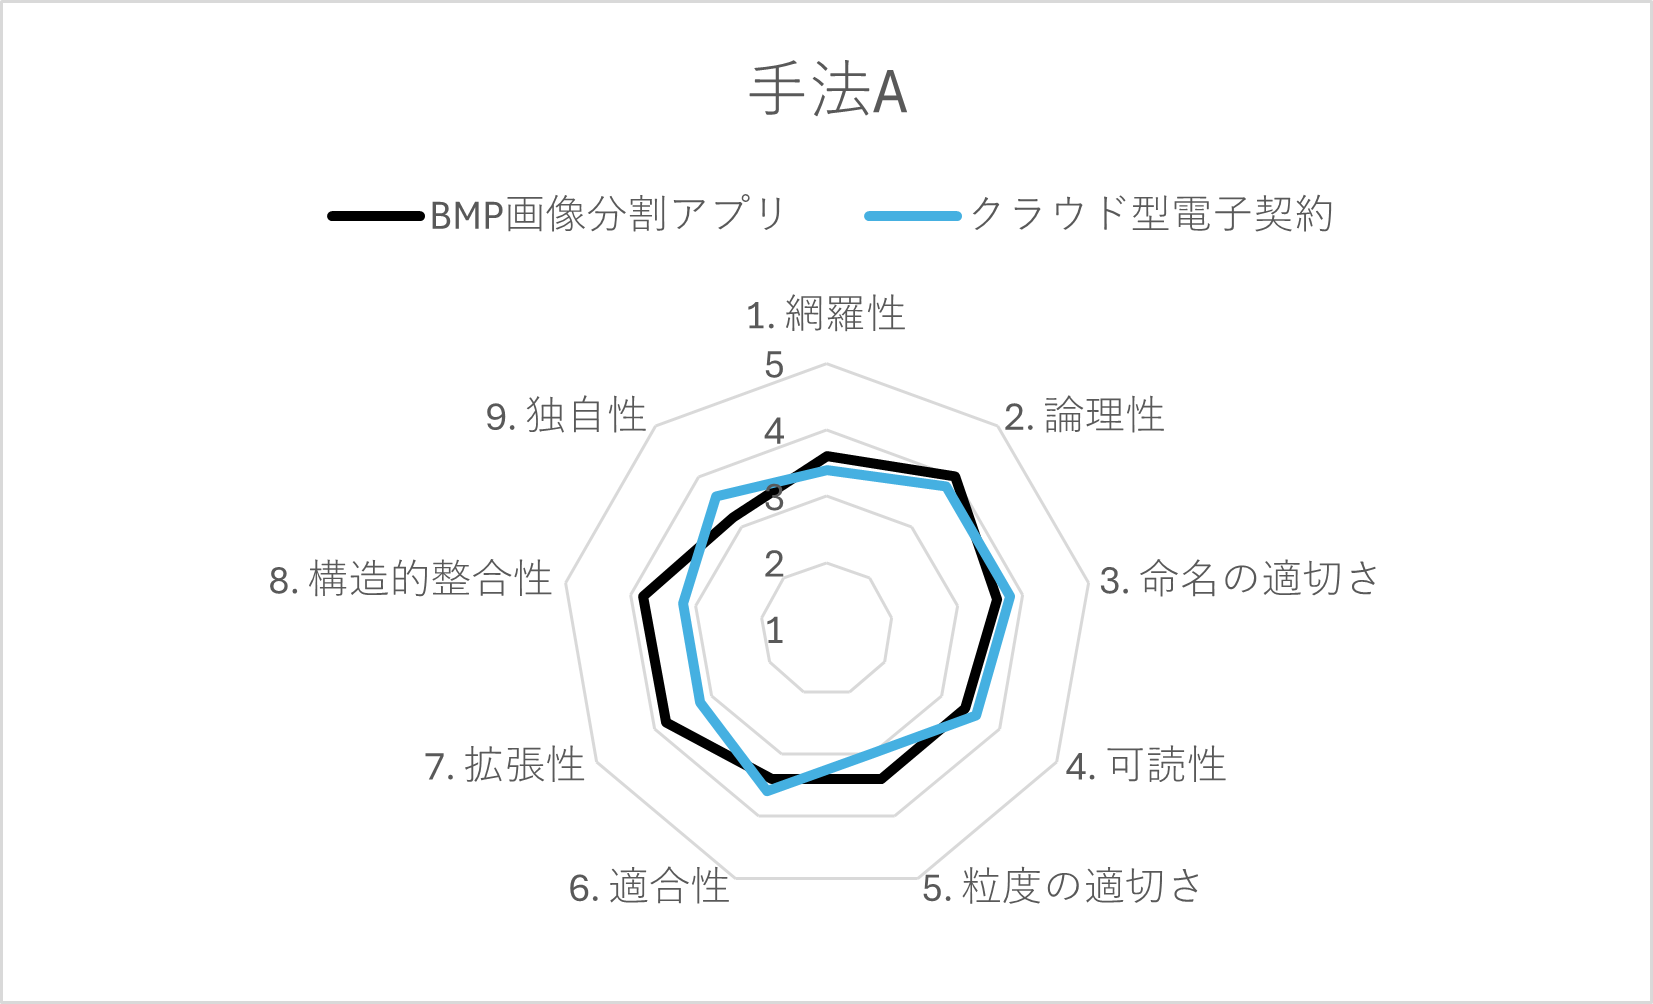
\includegraphics[width=0.8\textwidth]{images/手法Aばらつき.png}
    \caption{手法A(手動作成)の評価結果のばらつき}
    \label{fig:acomparison}
\end{figure}

図\ref{fig:bcomparison}に、手法B(自由プロンプト)のBMP画像分割アプリとクラウド型電子契約サービスの評価結果(表\ref{tb:bmp},表\ref{tb:cloud}参照)の比較を示す。
\begin{figure}[tp]
    \centering
    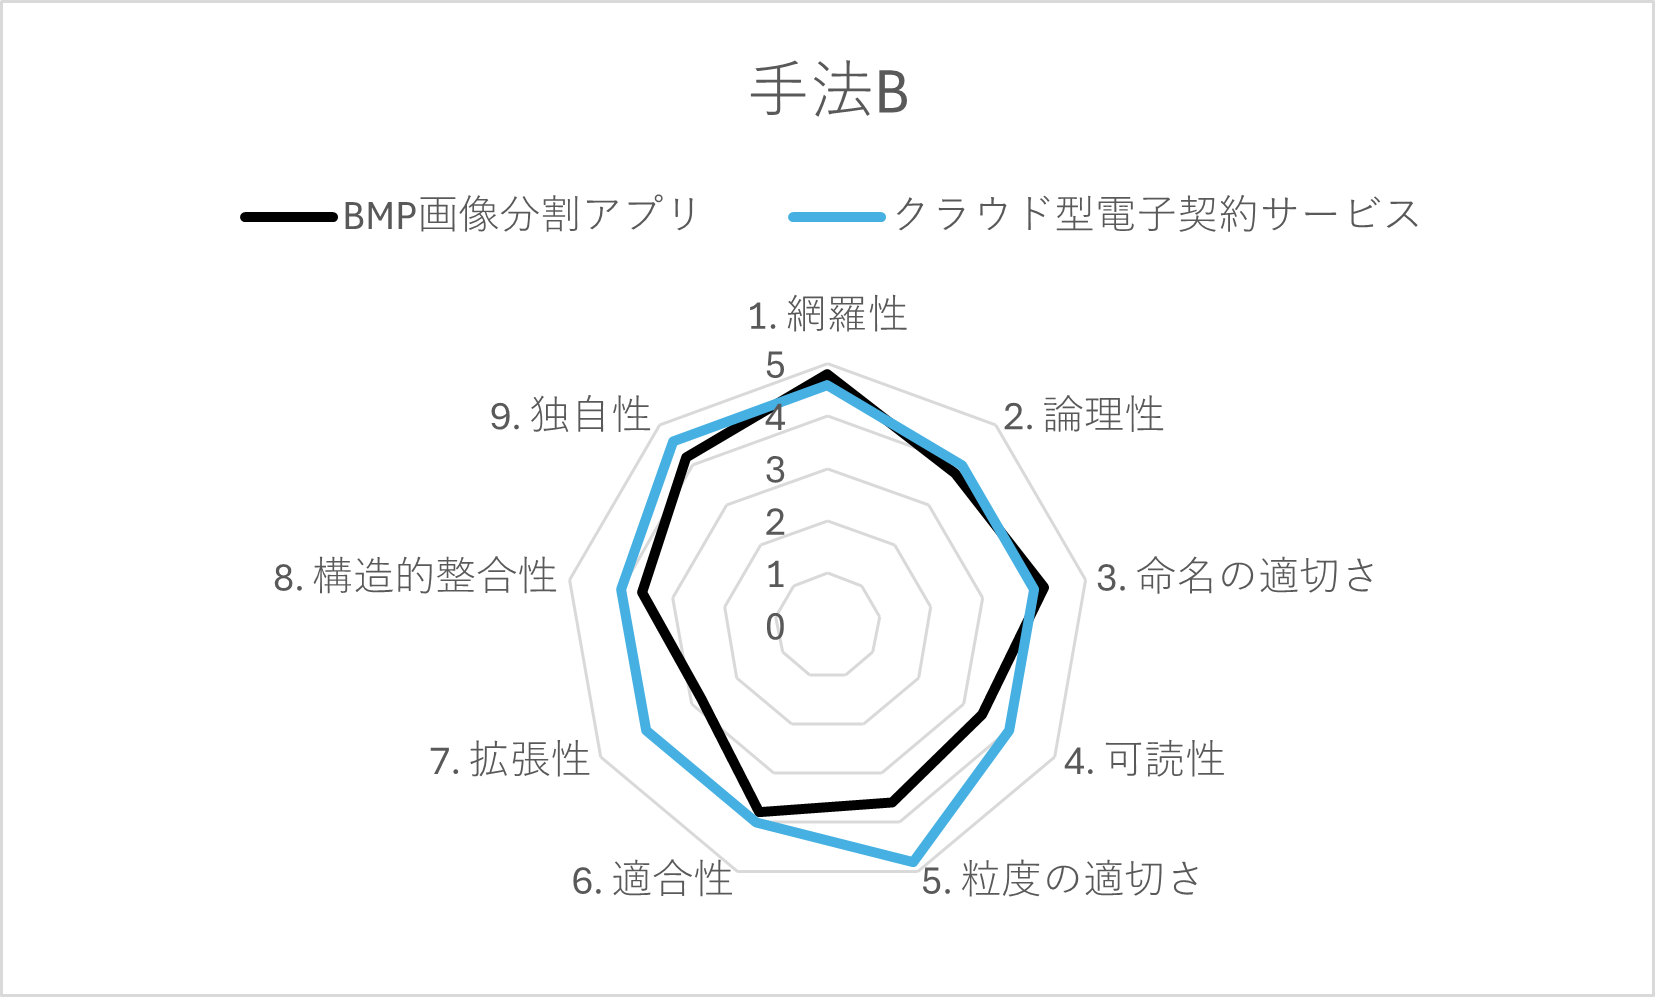
\includegraphics[width=0.8\textwidth]{images/手法Bばらつき.png}
    \caption{手法B(自由プロンプト)の評価結果のばらつき}
    \label{fig:bcomparison}
\end{figure}

図\ref{fig:ccomparison}に、手法C(提案プロンプト)のBMP画像分割アプリとクラウド型電子契約サービスの評価結果(表\ref{tb:bmp},表\ref{tb:cloud}参照)の比較を示す。
\begin{figure}[tp]
    \centering
    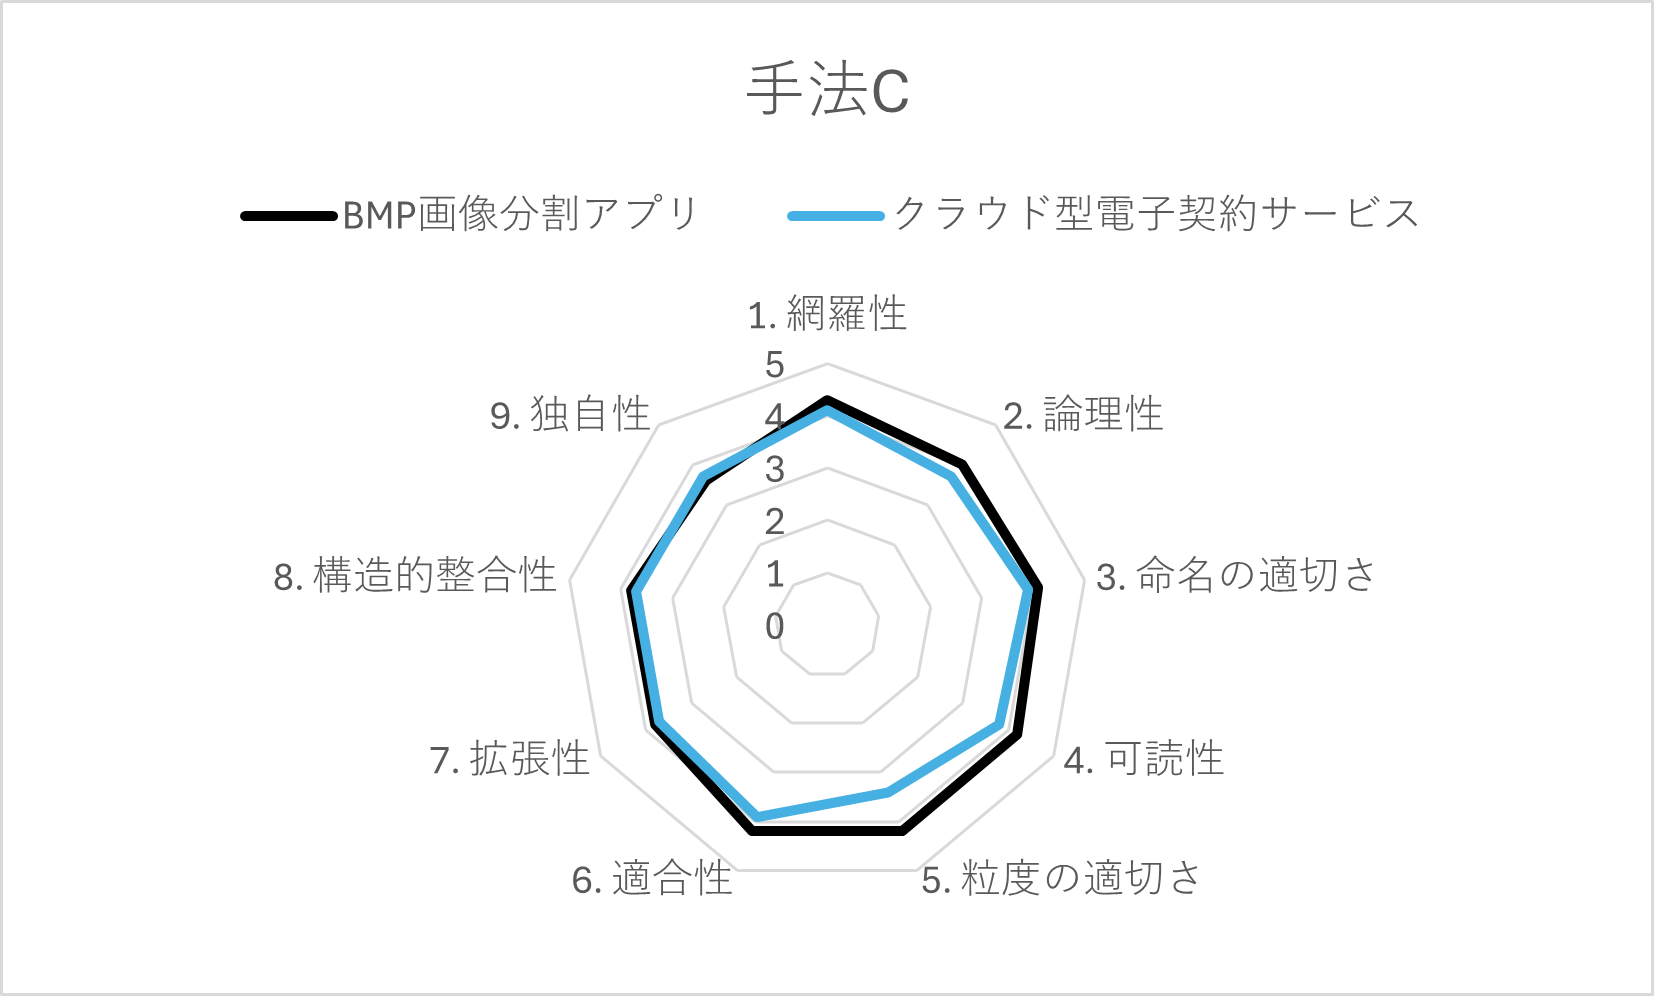
\includegraphics[width=0.8\textwidth]{images/手法Cばらつき.png}
    \caption{手法C(提案プロンプト)の評価結果のばらつき}
    \label{fig:ccomparison}
\end{figure}

図\ref{fig:acomparison}、図\ref{fig:bcomparison}、図\ref{fig:ccomparison}を比較すると、手法A、Bに比べ、手法Cは対象システムによる評価結果のばらつきが小さいことがわかる。

この結果は、手法B(自由プロンプト)は高い品質の章立てを出す可能性がある一方で、BMP画像分割アプリのような単純なシステムに対しては、冗長な構成が、拡張性、可読性の低下といったリスクにつながることを示している。
手法C(提案プロンプト)は、独自性や粒度の適切さでは自由プロンプトの最良ケースに劣るものの、対象とするシステムの複雑さが変わることによる章立ての品質のばらつきを抑えることができる点に特長があると言える。



また、単純なシステムであるBMP画像分割アプリにおいては、提案プロンプトは極めて有効に機能した。
手法C(提案プロンプト)の結果(表\ref{tb:detailed_evaluation_results_C}参照)は、網羅性4.4点、可読性4.4点、適合性4.4点と非常に高く、テンプレートが、小規模システムの全体像をカバーするのに十分であったことを示している。

一方、複雑なシステムであるクラウド型電子契約サービスにおいては、提案プロンプトの評価は総じて良好であったものの、項目によっては自由プロンプト(手法B(自由プロンプト))に劣る結果も見られた。

まず、提案プロンプトを用いた被験者間の評価結果のばらつきについて、被験者A(手法C(提案プロンプト))の粒度の適切さ(表\ref{tb:cloud_detailed_evaluation_results_C}参照)は2.8点と低く、被験者C(手法C(提案プロンプト))は4.0点であった。
同じプロンプトを使用しても、出力される粒度の適切さにばらつきが生じたことは、LLMの確率的な生成特性によるものと考えられる。

また、複雑なシステムでは、システム全体を俯瞰するだけでなく、個々の機能(ワークフロー図、排他制御など)について深い記述が求められるため、
手法C(提案プロンプト)のベースの章立てや制約では、LLMの生成能力を十分に引き出せない場合があると考えられる。

結論として、提案プロンプトはシステムの複雑さに関わらず「一定品質の保証」には寄与する。
しかし、複雑なシステムにおいて「高品質」かつ「高詳細」な章立てを目指す場合には、機能ごとに分割して生成する、あるいはChain-of-thoughtプロンプト\cite{chainofthought}を用いて章立てを段階的に出力していくといった、プロンプトエンジニアリングの更なる工夫が必要となる。

\section{まとめ}

本章の分析から、提案プロンプトについて、以下の3点が明らかになった。

\subsection{提案プロンプトの特長}
\label{sec:features_of_proposed_prompt}
提案プロンプトの最大の特長は、対象とするシステムの特性の違いによる章立ての品質のばらつきを抑制できる点である。

手法A(手動作成)との比較では、単純なシステム(BMP画像分割アプリ)における「項目の抜け漏れ」や、複雑なシステム(クラウド型電子契約サービス)における「ドメイン知識不足による独自性の欠如」といった、システムの特性ごとに生じやすい課題を、
役割付与とベース章立てテンプレート、出力指示(網羅性と自由度の指示)によって共通して補完できることを示した(表\ref{tb:bmp}、表\ref{tb:cloud}参照)。
特に、網羅性においてBMP画像分割アプリで手法A(手動作成)(3.6点)に対し、手法C(提案プロンプト)(4.3点)、
独自性においてクラウド型電子契約サービスで手法A(手動作成)(2.8点)に対し、手法C(提案プロンプト)(3.7点)と、システムの特性に関わらず改善した(表\ref{tb:bmp}、表\ref{tb:cloud}参照)。

手法B(自由プロンプト)との比較では、自由プロンプトがシステムの特性によって品質が大きく変動する(BMP: 34.2点、クラウド: 38.0点、差3.8点)のに対し、
提案プロンプトは対象システムが異なっても一定水準の品質(BMP: 36.2点、クラウド: 33.9点、差2.3点)であることを確認した(図\ref{fig:bcomparison}、図\ref{fig:ccomparison})。
自由プロンプトはクラウドサービスのような複雑なシステムでは高品質(粒度の適切さ4.8点、独自性4.6点)を達成する一方、単純なシステムでは過剰な詳細化などの問題が生じたが、
提案プロンプトは自由プロンプトと比較して、システムの特性に左右されにくいと言える。

\subsection{提案プロンプトの限界}
\label{sec:limitations_of_proposed_prompt}

提案プロンプトには、以下のトレードオフが存在することが明らかになった。

\begin{itemize}
    \item \textbf{網羅性と適合性}: システム仕様書の定義による制約は、適合性を高める(BMP: 4.2点、クラウド: 3.9点)代わりに、
    網羅性や独自性が低下する。これが、手法B(自由プロンプト)の最良ケースに劣る要因となっている。
    
    \item \textbf{網羅性と粒度の適切さ}: 出力指示(網羅性と自由度の指示)は網羅性を高める一方、
    階層が深くなりすぎて粒度の適切さの評価を下げる可能性がある。
    
    \item \textbf{テンプレートの制約}: ベース章立てテンプレートは命名の適切さを向上させるが、
    テンプレートに含まれない項目が生成されにくくなる可能性がある。
\end{itemize}

% これらのトレードオフは、提案するプロンプトが「システムの特性に依存しない汎用的な品質保証」を実現するための必然的な帰結である。
% 自由プロンプトが、対象システムに対するLLMの学習データ量やシステムとLLMの相性に依存して品質が大きく変動する「不確実性」を持つのに対し、提案するプロンプトは、あらゆるシステムに対して一定水準以上の網羅性と論理的構造を担保する「堅牢性」を備えている。
% すなわち、これは単なる妥協ではなく、実務において最も重要視される「品質の予測可能性と安定性」を、対象システムの規模や複雑さに関わらず提供できるという、本手法の核心的な価値を示している。

% これらのトレードオフは、提案するプロンプトが「品質の安定化」を優先した設計であることに起因する。
% すなわち、最高点を目指すのではなく、最低点を引き上げることに重点を置いた結果、
% 自由プロンプトの最良ケースには及ばないものの、安定した品質を実現している。

\subsection{提案プロンプトの適用場面の使い分け}

\ref{sec:features_of_proposed_prompt}節と\ref{sec:limitations_of_proposed_prompt}節の分析から、提案プロンプトの適用場面について、以下の示唆が得られる。

\textbf{提案プロンプトが特に有効な場面}
\begin{itemize}
    \item 仕様書作成の経験が浅いメンバーが作成する場合
    \item 小〜中規模のシステムで、標準的な構成が求められる場合
    \item 短時間で一定品質の章立てを確実に得たい場合
\end{itemize}

% \textbf{自由プロンプトとの併用を検討すべき場面}
\textbf{提案プロンプトの制約を緩める必要がある場面}
\begin{itemize}
    \item 複雑なシステムで、独自性が求められる場合
    \item LLMが豊富な知識を持つドメインのシステムで、その知識を最大限活用したい場合
    \item システム仕様書作成の経験と知識が豊富な作成者が、最高品質を目指す場合
\end{itemize}

このような使い分けにより、提案プロンプトの「品質の安定化」という強みを活かしつつ、
必要に応じて自由度を高めることで、より効果的な章立て生成が可能になると考える。

システムの複雑さに関する考察からは、以下の知見を得た。
単純なシステム(BMP画像分割アプリ)においては、提案プロンプトは極めて有効に機能し、網羅性4.4点、可読性4.4点、適合性4.4点と非常に高い評価を得た。
これは、テンプレートが小規模システムの全体像をカバーするのに十分であったことを示している。

一方、複雑なシステム(クラウド型電子契約サービス)においては、提案プロンプトは総じて良好な評価を得たものの、
同一のプロンプトを使用しているにも関わらず、生成された章立ての「粒度の適切さ」において評価にばらつきが生じる結果となった(被験者A: 2.8点、被験者C: 4.0点)。
これは、同じ制約とテンプレートを与えても、複雑なシステムにおいてはLLMの出力の品質が生じやすく、完全に品質を均一化することの難しさを示唆している。
複雑なドメインでは、個々の機能について深い記述が求められるため、
画一的なテンプレートや制約だけでは、LLMの生成能力を十分に引き出せない場合がある。

したがって、複雑なシステムにおいては、提案プロンプトをベースとしつつ、
Chain-of-thoughtプロンプト\cite{chainofthought}を取り入れ、機能ごとに分割して生成する、あるいは、
網羅的な章立てを生成してから、章立てテンプレートに沿って整形していくといった、
段階的なアプローチが有効である可能性があると結論付ける。
